\section{What about the remaining terms and the C.L divergence paradox }

In \ref{chap:pseudoturbulence} we demonstrated that the Reynolds stress tensor could be expressed as,
\begin{equation}
    \avg{\chi_f \textbf{u}_f'\textbf{u}_f'}
    = 
    \phi_f
    \int_{\mathbb{R}^3}
    \textbf{v}_f^\text{nst}
    \textbf{v}_f^\text{nst}
    P_\text{nst}^f
    d\textbf{r}
    + 
    \phi_f
    \int_{\mathbb{R}^3}
    \textbf{v}_f^\text{nst}
    \textbf{v}_f^\text{nst}
    P_\text{nst}^f
    d\textbf{y}
    + 
    \int_{\mathbb{R}^3}
    \avg{
        \chi_f
        \textbf{u}_f''
        \textbf{u}_f''
        % \sum_i 
        % \delta(\textbf{x}+\textbf{y}-\textbf{x}_i)
        % \delta(\textbf{w}-\textbf{u}_i)
        % h_i
        \delta_\text{nst}
    }
    d\textbf{y}.
    \label{ap:eq:relation_ensemble_nst}
\end{equation}
For the sake of simplicity, in this appendix we consider that all droplets posses the same center of mass velocity $\textbf{u}_p$. 
Although the first term on the RHS can be computed at $\mathcal{O}(\phi)$ (see \ref{chap:pseudoturbulence}) no justifications have been provided to ensure that the second term could be neglected. 
In this appendix we demonstrate that, (1) the nearest particles' statistics formulation of the Reynolds stress \eqref{ap:eq:relation_ensemble_nst} leads to the same results as \citet{caflisch1985variance} if one consider the presence of the second term, and (2) that for periodic domain containing several droplets/particles, only the averaged wake of the nearest neighbor is predominant on the final result. 


\subsection{Zhang's idea}

\begin{equation}
    \avg{\textbf{u}'\textbf{u}'}
    =
    \int_{\mathbb{R}^3}\avg{\textbf{u}'\textbf{u}'\delta_{nst}} d\textbf{r}
\end{equation}
then derive directly an equation for $\textbf{u}'$ or $\textbf{u}_f'$. 

So i need $\textbf{u}^0\textbf{u}^0\delta_{nst}$ to which i subtract the equation for $\textbf{u} \textbf{u}$
that is to be computed with 
\begin{align}
    \label{eq:dt_rhou_k2}
    \pddt [\rho_k/2(u_k^0)^2]  
    + \div [\rho_k/2(u_k^0)^2\textbf{u}_k^0 - \textbf{u}_k^0 \cdot \bm{\sigma}_k^0]
    &=
    \rho_k\textbf{u}_k^0 \cdot \textbf{g}  
    -  \bm{\sigma}_k^0 : \grad \textbf{u}_k^0,
    \\
    \label{eq:dt_rhoe_k}
    \pddt (\rho_ke_k^0)  
    + \div (
        \rho_ke_k^0\textbf{u}_k^0
        + \textbf{q}_k^0
        )
    &= 
    \bm{\sigma}_k^0 : \grad \textbf{u}_k^0,
\end{align} 



\subsection{Contribution of the second-nearest droplet}

Using similar method to what is done for \ref{ap:eq:relation_ensemble_nst} we may demonstrate that,  
\begin{align*}
    \avg{\chi_f \textbf{u}_f'\textbf{u}_f'}[\textbf{x},t]
    &= 
    \int_{\mathbb{R}^3}
    \avg{\chi_f \textbf{u}_f'\textbf{u}_f' 
    \sum_i^N \delta(\textbf{x}_i - \textbf{x}- \textbf{r}_1)
    h_i
    }
    d\textbf{r}_1\\
    &= 
    \int_{\mathbb{R}^3}
    \int_{\mathbb{R}^3}
    \avg{\chi_f \textbf{u}_f'\textbf{u}_f' 
    \sum_i^N \delta(\textbf{x}_i - \textbf{x}- \textbf{r}_1)
    h_i
    \sum_{j\neq i}^N \delta(\textbf{x}_j - \textbf{x}- \textbf{r}_2)
    h_j
    }
    d\textbf{r}_2
    d\textbf{r}_1
\end{align*}
Doing so we arrive at the conslusion that, 
\begin{multline}
    \avg{\chi_f \textbf{u}_f'\textbf{u}_f'}
    = 
    \phi_f
    \int_{\mathbb{R}^3}
    \textbf{v}_f^\text{nst}
    \textbf{v}_f^\text{nst}
    P_\text{nst}^f
    d\textbf{r}_1
    + 
    \phi_f
    \int_{\mathbb{R}^6}
    \textbf{v}_f^\text{2-nst}
    \textbf{v}_f^\text{2-nst}
    P_\text{2-nst}^f
    d\textbf{r}_1
    d\textbf{r}_2 \\
    + 
    \int_{\mathbb{R}^6}
    \avg{
        \chi_f
        \textbf{u}_f'''
        \textbf{u}_f'''
        % \sum_i 
        % \delta(\textbf{x}+\textbf{y}-\textbf{x}_i)
        % \delta(\textbf{w}-\textbf{u}_i)
        % h_i
        \delta_\text{nst}
    }
    d\textbf{r}_1
    d\textbf{r}_2.
\end{multline}
where we have introduced the following notation, 
\begin{align}
    \phi_f
    &= 
    \avg{\chi_f}\\
    \phi_f P_\text{nst}^f 
    &= 
    \avg{\chi_f  
    \sum_i^N \delta(\textbf{x}_i - \textbf{x}- \textbf{r})
    h_i
    }\\
    \phi_f P_\text{nst}^f \textbf{u}_f^\text{nst}
    &= 
    \avg{\chi_f  
    \sum_i^N \delta(\textbf{x}_i - \textbf{x}- \textbf{r})
    h_i
    }\\
    \phi_f P_\text{2-nst}^f
    &= 
    \avg{\chi_f  
    \sum_i^N \delta(\textbf{x}_i - \textbf{x}- \textbf{r})
    h_i
    \sum_{j\neq i}^N \delta(\textbf{x}_j - \textbf{x}- \textbf{r})
    h_j
    }\\
    \phi_f P_\text{2-nst}^f \textbf{u}_f^\text{2-nst}
    &= 
    \avg{\chi_f \textbf{u}_f^0 
    \sum_i^N \delta(\textbf{x}_i - \textbf{x}- \textbf{r})
    h_i
    \sum_{j\neq i}^N \delta(\textbf{x}_j - \textbf{x}- \textbf{r})
    h_j
    }
\end{align}
where $P_\text{2-nst}^f[\textbf{r}_1, \textbf{r}_2|\textbf{x}]$ is the probability of finding the center of mass of the two nearest droplets to the point $\textbf{x}$ (being occupied by the continuous phase) at the location $\textbf{r}_1$ and $\textbf{r}_2$.  

Additionally, we introduce the disturbance velocity fields, 
\begin{align}
    \textbf{v}^\text{nst-f}_f[\textbf{r}_1,\textbf{x}] &= \textbf{u}^\text{nst-f}_f - \textbf{u}_f\\
    \textbf{v}^\text{2-nst-f}_f[\textbf{r}_1,\textbf{r}_2,\textbf{x}] &= \textbf{u}^\text{2-nst-f}_f - \textbf{u}_f^\text{nst-f}\\
    \textbf{v}'''_f &= \textbf{u}^0_f - \textbf{u}^\text{2-nst-f}_f
\end{align}
As discussed in the body of the text it is also useful to consider the bulk velocity evaluated at an arbitrary point \textbf{z}, knowing that the continuous phase is present at \textbf{x} and that the nearest neighbor to this point is present at $\textbf{r}_1$, and eventually that a second-nearest neighbor is present at $\textbf{r}_2$. 
Therefore, we introduce the fields, 
\begin{align}
    \textbf{v}^\text{nst-f}[\textbf{z}| \textbf{r}_1,\textbf{x}] &= \textbf{u}^\text{nst} - \textbf{u}\\
    \textbf{v}^\text{2-nst-f}[\textbf{z}| \textbf{r}_1,\textbf{r}_2,\textbf{x}] &= \textbf{u}^\text{2-nst} - \textbf{u}^\text{nst}\\
\end{align}
The alternative definitions of these fields are, 
\begin{align}
    P_\text{nst-f}^f \textbf{v}^\text{nst-f} &= \avg{ \textbf{u}^0 \left[\chi_f \sum_i^N \delta(\textbf{x}_i - \textbf{x}- \textbf{r})h_i - P_\text{nst}^f\right]}\\
    P_\text{2-nst-f}^f \textbf{v}^\text{2-nst-f} &= \avg{ \textbf{u}^0 \chi_f \sum_i^N \delta(\textbf{x}_i - \textbf{x}- \textbf{r})h_i \left[\sum_{j\neq i}^N \delta(\textbf{x}_j - \textbf{x}- \textbf{r}) h_j  - P_\text{2-nst}^\text{nst-f} \right] }
\end{align}
where $P_\text{2-nst}^\text{nst-f}$ is the probability of finding the second-nearest neighbor to \textbf{x} at $\textbf{r}_2$ knowing that the first nearest neighbor is already at $\textbf{r}_1$. 
For sake of brevity we introduce the notations, 
\begin{align}
    \delta_\text{nst-f}[\FF,t,\textbf{x},\textbf{r}_1] &\to \chi_f \sum_i^N \delta(\textbf{x}_i - \textbf{x}- \textbf{r})h_i \\
    \delta_\text{2-nst-f}[\FF,t,\textbf{x},\textbf{r}_1,\textbf{r}_2]  &\to  \chi_f \sum_i^N \delta(\textbf{x}_i - \textbf{x}- \textbf{r}_1)h_i \sum_{j\neq i}^N \delta(\textbf{x}_j - \textbf{x}- \textbf{r}_2) h_j  \\
    \delta_\text{nst-f}'[\FF,t,\textbf{x},\textbf{r}_1] &\to \chi_f \sum_i^N \delta(\textbf{x}_i - \textbf{x}- \textbf{r})h_i - P_\text{nst}^f\\
    \delta_\text{2-nst-f}'[\FF,t,\textbf{x},\textbf{r}_1,\textbf{r}_2]  &\to  \chi_f \sum_i^N \delta(\textbf{x}_i - \textbf{x}- \textbf{r}_1)h_i \left[\sum_{j\neq i}^N \delta(\textbf{x}_j - \textbf{x}- \textbf{r}_2) h_j  - P_\text{2-nst}^\text{nst-f} \right]
\end{align}
With this notation note that, 
\begin{align}
    \avg{\delta_\text{2-nst-f}'} &= 0\\
    P_\text{2-nst-f} \textbf{v}^\text{2-nst-f} &= \avg{\delta_\text{2-nst-f}' \textbf{u}^0}\\
    P_\text{2-nst-f} (\phi_f^\text{2-nst-f} -\phi_f^\text{nst-f}) &= \avg{\delta_\text{2-nst-f}' \chi_f}= - \avg{\delta_\text{2-nst-f}' \chi_d}= - P_\text{2-nst-f} (\phi_d^\text{2-nst-f} -\phi_d^\text{nst-f})
\end{align} 
The methodology to derive the mass and momentum equations governing $\textbf{v}^\text{nst}$ and $\textbf{v}^\text{2-nst}$ is then clear, we multiply the local single-fluid formulation of the momentum equation evaluated at a point \textbf{z} by $\delta_\text{2-nst-f}'$ or $\delta_\text{nst-f}'$, and ensemble average the resulting equations. 

In Stokes regime the single fluid formulation of the mass and momentum equations reads as, 
\begin{align}
    \div \textbf{u}^0 & =0 \\
    \div (\chi_f \bm\sigma_f^0 + \chi_d \bm\sigma_d^0 + \delta_\Gamma \bm\sigma_\Gamma^0)
    &=
    - (\chi_d \rho_d + \chi_f \rho_f) \textbf{g}
\end{align}
Averaging gives, 
\begin{align}
    \div \avg{\delta_\text{2-nst-f}' \textbf{u}^0} & =0 \\
    \div \avg{\delta_\text{2-nst-f}' (\chi_f \bm\sigma_f^0 + \chi_d \bm\sigma_d^0 + \delta_\Gamma \bm\sigma_\Gamma^0)}
    &=
    - \avg{\delta_\text{2-nst-f}'(\chi_d \rho_d + \chi_f \rho_f) \textbf{g}}
\end{align}

Then, noticing that, 
\begin{align*}
    \avg{\delta_\text{2-nst-f}' \chi_f \bm\sigma_f^0}
    =&
    -  P^f_\text{2-nst-f} \tau^\text{2-nst-f}_f \bm\delta
    + \mu_f P^f_\text{2-nst-f} \left[
        \grad \textbf{v}^\text{2-nst-f}
        + (\grad \textbf{v}^\text{2-nst-f})^\dagger
    \right]\\
    &- \avg{ \chi_d \delta_\text{2-nst-f}'\textbf{e}_d^0 } 
    % +  P^f_\text{2-nst-f} (\phi_d^\text{2-nst-f} p^\text{2-nst-f}_f - \phi_d^\text{nst-f} p^\text{nst-f})
    + \avg{\chi_d (p^\text{2-nst-f}_f \delta_\text{2-nst-f} - \delta_\text{nst-f}P_\text{2-nst}^\text{nst-f} p^\text{nst-f}_f )}\\
    \avg{\delta_\text{2-nst-f}'(\chi_d \rho_d + \chi_f \rho_f)}
    &=
    \avg{\delta_\text{2-nst-f}'\chi_d (\rho_d - \rho_f)}
\end{align*}
where $\tau^\text{2-nst}_f = p_f^\text{2-nst-f} - p_f^\text{nst-f}$ is the disturbance pressure field. 
For any tensor $\textbf{A}$ appearing under the divergence sign in the momentum equation we may write 
\begin{equation}
    \div\avg{\chi_d \textbf{A}}
    =
    \div\pOavg{\textbf{A}}
    -\frac{1}{2} \grad\grad : \pOavg{\textbf{Ar}+\textbf{rA}}
\end{equation}
Additionally, any integral of the stress, or moments of the stress may be written as, 
\begin{align*}
    \intO{
        \bm\sigma_d^0
    }
    + 
    \intS{
        \bm\sigma_\Gamma^0
    }
    &=
    \intS{\textbf{r}\bm\sigma_f^0 \cdot \textbf{n}}\\
    \intO{
        \textbf{r}\bm\sigma_d^0+ \textbf{r}\bm\sigma_d^0
    }
    + 
    \intS{
        \textbf{r}\bm\sigma_\Gamma^0+\textbf{r}\bm\sigma_\Gamma^0
    }
    &=
    \intS{\textbf{rr}\bm\sigma_f^0 \cdot \textbf{n}}
    + 
    \rho_d \intO{\textbf{rr}}
\end{align*}

Using this formulation for the stresses tensors and also for the pressure and internal shear tensor we arrive at the conclusion that, 
\begin{align}
    P_\text{2-nst-f}\div \textbf{u}^\text{2-nst-f} & =0 \\
    P_\text{2-nst-f}\div \bm\Sigma^\text{2-nst-f}
    &=
    P_\text{2-nst-f}\div \bm\sigma^\text{2-nst-f}_\text{eff}
    - \avg{\delta_\text{2-nst-f}'\delta_p  (\rho_d - \rho_f) \intO{}}
\end{align}
with the effective stress defined as, 
\begin{multline}
    \bm\sigma^\text{2-nst-f}_\text{eff}
    =
    - \avg{\delta_p \delta_\text{2-nst-f}'\intS{\textbf{r}\bm\sigma_f^0 \cdot \textbf{n}}}
    + \avg{\delta_p \delta_\text{2-nst-f}' \intO{\textbf{e}_d^0} }  \\
    -\bm\delta \avg{\delta_p \left(\intO{p^\text{2-nst-f}_f }\delta_\text{2-nst-f} - \delta_\text{nst-f}P_\text{2-nst}^\text{nst-f} \intO{p^\text{nst-f}_f} \right)}\\
    + \frac{1}{2}\div \left[
        \avg{\delta_p \delta_\text{2-nst-f}'\intS{\textbf{rr}\bm\sigma_f^0 \cdot \textbf{n}}}
        + \avg{\delta_p \delta_\text{2-nst-f}'\rho_f \intO{\textbf{rr}}}
    \right]\\
    + \frac{1}{2}\div \left[
        - \avg{\delta_p \delta_\text{2-nst-f}' \intO{\textbf{r}\textbf{e}_d^0+ \textbf{e}_d^0 \textbf{r}} }  \right. \\ \left. 
        - \avg{\delta_p \left(\intO{p^\text{2-nst-f}_f (\textbf{r}\bm\delta + \bm\delta \textbf{r})}\delta_\text{2-nst-f} - \delta_\text{nst-f}P_\text{2-nst}^\text{nst-f} \intO{p^\text{nst-f}_f (\textbf{r}\bm\delta + \bm\delta \textbf{r})} \right)}
    \right]
\end{multline}

\begin{align}
    P_\text{2-nst-f}[\textbf{r}_2,\textbf{r}_1,\textbf{x}]
    &= 
    P_\text{nst-f}[\textbf{r}_1,\textbf{x}]
    P_\text{2-nst-f}[\textbf{r}_2|\textbf{r}_1,\textbf{x}]
    = 
    \phi_f[\textbf{x}]
    P_\text{nst-f}[\textbf{r}_1|\textbf{x}]
    P_\text{2-nst-f}[\textbf{r}_2|\textbf{r}_1,\textbf{x}]\\
    P_\text{2--f}[\textbf{r}_2,\textbf{r}_1,\textbf{x}]
    &= 
    P_\text{1-f}[\textbf{r}_1,\textbf{x}]
    P_\text{2-f}[\textbf{r}_2|\textbf{r}_1,\textbf{x}]
    = 
    \phi_f[\textbf{x}]
    P_\text{1-f}[\textbf{r}_1|\textbf{x}]
    P_\text{2-f}[\textbf{r}_2|\textbf{r}_1,\textbf{x}]
\end{align}
Additionally, following \citet{zhang2021ensemble} we may now introduce, 
\begin{align}
    h_\text{1-nst}[\textbf{r}_1, \textbf{x}]
    =
    P_\text{nst-f}[\textbf{r}_1 , \textbf{x}] / P_\text{1-f}[\textbf{r}_1 ,\textbf{x}]
    = 
    P_\text{nst-f}[\textbf{r}_1 | \textbf{x}] /P_\text{1-f}[\textbf{r}_1 |\textbf{x}]
\end{align}
where $h_\text{2-nst}[\textbf{r}_1, \textbf{x}]$ is the probability of finding no particles center of mass in the spherical shell $a < |\textbf{z} - \textbf{x}| < |\textbf{r}_1 - \textbf{x}|$. 
Similarly
\begin{align}
    h_\text{2-nst}[\textbf{r}_2,\textbf{r}_1, \textbf{x}]
    =
    P_\text{2-nst-f}[\textbf{r}_2 ,\textbf{r}_1 , \textbf{x}] / P_\text{2-f}[\textbf{r}_2 ,\textbf{r}_1 ,\textbf{x}]
    =
    P_\text{2-nst-f}[\textbf{r}_2 |\textbf{r}_1 , \textbf{x}] 
    / 
    P_\text{2-f}[\textbf{r}_2 |\textbf{r}_1 ,\textbf{x}]
    h_\text{1-nst}
\end{align}
where $h_\text{2-nst}[\textbf{r}_2,\textbf{r}_1, \textbf{x}]$ is the probability that $\textbf{r}_1$ and $\textbf{r}_2$ are the nearest particles to \textbf{x}, knowing both particles are present and fluid at \textbf{x}. 
In other worlds it is the probability that no-other particles are present in the spherical shell $a < |\textbf{z} - \textbf{x}| < |\textbf{r}_1 - \textbf{x}|$ excluding the volume that the first particle occupy. 

Finally, 
\begin{equation}
    P_\text{2-nst-f}[\textbf{r}_2 ,\textbf{r}_1 , \textbf{x}] 
    =
    h_\text{2-nst}[\textbf{r}_2,\textbf{r}_1, \textbf{x}] 
    / h_\text{1-nst}[\textbf{r}_2,\textbf{r}_1 ]
    P_\text{2-f}[\textbf{r}_2 ,\textbf{r}_1 ,\textbf{x}]
\end{equation}
\paragraph*{Second option (may be better): }

\begin{equation}
    h_2[\textbf{r}_2,\textbf{r}_1,\textbf{x}]
    = 
    P_\text{2-nst-f}[\textbf{r}_2|\textbf{r}_1,\textbf{x}]
    / 
    P_\text{2-f}[\textbf{r}_2|\textbf{r}_1,\textbf{x}]
\end{equation}
So that $h_2$ is the probability of finding no particle for the points \textbf{z} in the region $|\textbf{r}_1- \textbf{x}|<|\textbf{z}- \textbf{x}|<|\textbf{r}_2- \textbf{x}|$, making the particle 2 the second closested. 



\paragraph*{Summary}

\begin{equation}
    P_\text{2-nst-f}
    = 
    \phi_f 
    P_\text{nst-f}
    P_\text{2-nst-f}
    = 
    \phi_f 
    h_1 P_\text{1-f}
    h_2 P_\text{2-f}
\end{equation}
In the dilute regime where there is no overlap it is easy to compute all of these terms. 


To compute the probability $h_1$ it is easy. 
It is one minus th proba of finding a particle in the volume $V$. 
In that case the volume is, 
\begin{equation}
    V = \frac{4}{3}\pi (r_1^3 - a^3)
\end{equation}
then we introduce the infinitesimal volume $dv = V / N$. The probability of finding a part in sucha small volume is $n_p v$ and thus, 
\begin{equation}
    h_1 
    = \lim_{N\to\infty}
    (1-n_p \frac{V}{N})^N 
    = e^{-n_p V}
\end{equation}

\begin{tikzpicture}

    % Define points
    \coordinate (X) at (0,0); % Center X
    \coordinate (r1) at (3,0); % Point r1
    \coordinate (r2) at (2.6,3); % Point r2 (farther than r1)

    % Dashed circles centered at X
    \draw[dashed] (X) circle (1); % Dashed circle from X to r1
    \draw[dashed] (X) circle (3); % Dashed circle from X to r1
    \draw[dashed] (X) circle (4); % Dashed circle from X to r2
    \draw[dashed] (r1) circle (2); % Dashed circle from X to r2

    % Solid circle centered at r1 with radius 2a
    \draw[thick] (r1) circle (2);

    % Shaded region between r1 and r2, excluding the solid circle
    \begin{scope}
        \clip (r1) circle (2);
        % \fill (X) circle (6);
    \end{scope}

    % Draw labels
    \fill (X) circle (2pt) node[left] {\Large $\textbf{x}$};
    \fill (r1) circle (2pt) node[below] {\Large $\textbf{r}_1$};
    \fill (r2) circle (2pt) node[below] {\Large $\textbf{r}_2$};

\end{tikzpicture}

The same reasoning can be made for $h_2$ except that the volume in question is, 
\begin{equation}
    V = \{
        |\textbf{r}_1 - \textbf{x}| < |\textbf{z} - \textbf{x}| < |\textbf{r}_2 - \textbf{x}|
        \setminus
        |\textbf{z} - \textbf{r}_1| < 2a
    \}
\end{equation}
For consistness we intriducde 
\begin{equation}
    V = \{
        r_1 < |\textbf{z} - \textbf{x}| < r_2
        \setminus
        |\textbf{z} - \textbf{r}_1| < 2a
    \}
\end{equation}
We must find the volume of the spherical caps. 
The volume of the spherical shell excluding the sphere at $\textbf{r}_1$ can be computed as, 
\begin{equation}
    V 
    = 
    \int_0^{2\pi}
    \int_{r_1}^{r_2}
    \int_{\theta_{min}(r)}^{\pi}
    r^2
    \sin\theta
    d\theta 
    dr
    d\varphi
\end{equation}
where we have choosen a local coordinate system centered at $\textbf{x}$ in the direction of $\textbf{r}_1$. 
In this situation the eq of the surface of the sphere at $\textbf{r}_1$ might be written, 
\begin{align}
    x^2
    + y^2
    + (z-r_1)^2
    &= (2a)^2\\
    r^2 \sin^2\theta_{min}
    + (r \cos\theta_{min} -r_1)^2
    &= (2a)^2\\
    - r^2 
    + 2 \cos\theta_{min} r r_1 
    - r_1^2
    &= - (2a)^2\\
    + 2 \cos\theta_{min} r r_1 
    &= 
    r^2 
    + 
    (r_1+2a)(r_1-2a)
\end{align}
Thus, 
\begin{equation}
    \theta_{min}
    = \left\{
    \begin{tabular}{ll}
        $\arccos\{
        \frac{
            r^2 
            + r_1^2
             - (2a)^2
        }{2 r r_1}\}
        $&$
        \forall r < (r_1+2a)$\\
        $ 
        0
        $&$
        \forall r > (r_1+2a)$
    \end{tabular}
    \right.
\end{equation}


So for points $r_2 <r_1 +2a$ the integration goes like, 
\begin{align}
    V 
    &= 
    \int_0^{2\pi}
    d\varphi
    % \left[
    \int_{r_1}^{r_2}
    \int_{\theta_{min}(r)}^{\pi}
    % +
    %     \int_{r_1+2a}^{r_2}
    %     \int_{0}^{\pi}
    % \right]
    r^2
    \sin\theta
    d\theta 
    dr\\
    &= 
    \pi /r_1
    \int_{r_1}^{r_2} 
    [2r^2r_1 +  
        r^3 
        + r(r_1^2
        - (2a)^2)
    ]
    dr\\
    &= 
    \pi /r_1
    [2r^3/3r_1 
        +  r^4/4
        + r^2/2 (r_1^2 - (2a)^2)
    ]_{r_1}^{r_2} \\
    &= 
    \pi /r_1
    [\frac{2r_1}{3}(r_2^3-r_1^3) 
    + \frac{1}{4} (r_2^4-r_1^4)
        + \frac{1}{2}(r_2^2 - r_1^2) (r_1^2 - (2a)^2)]\\
    & = \frac{4\pi}{3}
    \frac{ 
     8 r_{1} \left(r_{2}^{3} - r_{1}^{3}\right) 
    + 3 (r_{2}^{4} - r_{1}^{4})
    + 6  \left(r_{1}^{2} - (2 a)^{2} \right) \left(r_{2}^{2} - r_{1}^{2}\right)}{16 r_{1}}
\end{align}

For points $r_2 > r_1 +2a$ we have, 
\begin{align}
    V &= 
    \pi /r_1
    [\frac{2r_1}{3}((r_1 + 2a)^3-r_1^3) 
    + \frac{1}{4} ((r_1 + 2a)^4-r_1^4)
        + \frac{1}{2}((r_1 + 2a)^2 - r_1^2) (r_1^2 - (2a)^2)]
    \\
    &+\frac{4\pi}{3}(r_2^3 - (r_1+(2a)^3))\\
    &
    =
    \frac{4\pi}{3}\left[
        -\frac{3a^4}{r_1}
        - 4 a^3 
        + r_2^3
        -r_1^3
    \right]
\end{align}

Assuming $r_1/a \to r_1$ and $r_2/a \to r_2$ we have, 
\begin{align}
    V 
    &= 
    \frac{4\pi a^3}{3}
    \frac{ 
     8 r_{1} \left(r_{2}^{3} - r_{1}^{3}\right) 
    + 3 (r_{2}^{4} - r_{1}^{4})
    + 6  \left(r_{1}^{2} - 4 \right) \left(r_{2}^{2} - r_{1}^{2}\right)}{16 r_{1}}
    \\
    V 
    &= 
    \frac{4\pi a^3}{3}\left[
        -\frac{3}{r_1}
        - 4 
        + r_2^3
        -r_1^3
    \right]
\end{align}



We conclude that, 
\begin{align}
    h_1 &= \exp\left\{-\phi (r_1^3 - 1)\right\}& \forall r_1 > a\\
    h_2 &= \exp\left\{-\phi 
        \frac{ 
        8 r_{1} \left(r_{2}^{3} - r_{1}^{3}\right) 
       + 3 (r_{2}^{4} - r_{1}^{4})
       + 6  \left(r_{1}^{2} - 4 \right) \left(r_{2}^{2} - r_{1}^{2}\right)}{16 r_{1}}
    \right\} &\forall  r_2 < r_1 + 2\\ 
    h_2 &= \exp\left\{-\phi 
    \left[
        -\frac{3}{r_1}
        - 4 
        + r_2^3
        -r_1^3
    \right]
    \right\} &\forall  r_2 > r_1 + 2 
\end{align}

\paragraph*{Results : }
For the $r_2 < r_1 + 2$ we have, 
\begin{equation}
    P_{2-nst}^f[\textbf{r}_2 | \textbf{r}_1,\textbf{x}]
    = 
    n_p[\textbf{r}_2]
    \exp\left\{-\phi 
        \frac{ 
        8 r_{1} \left(r_{2}^{3} - r_{1}^{3}\right) 
       + 3 (r_{2}^{4} - r_{1}^{4})
       + 6  \left(r_{1}^{2} - 4 \right) \left(r_{2}^{2} - r_{1}^{2}\right)}{16 r_{1}}
    \right\} 
\end{equation}
and for $r_2 > r_1 + 2$
\begin{equation}
    P_{2-nst}^f[\textbf{r}_2 | \textbf{r}_1,\textbf{x}]
    = 
    n_p[\textbf{r}_2]
    \exp\left\{-\phi 
    \left[
        -\frac{3}{r_1}
        - 4 
        + r_2^3
        -r_1^3
    \right]
    \right\} 
\end{equation}
and for both cases $P_{2-nst}^f = 0 $ for $r_2 < r_1$ and $|\textbf{r}_2-\textbf{r}_1|<2a$. 
Note that we should have 
\begin{equation}
    \int_{
        r_1 < r_2
        \setminus
        |\textbf{r}_2 - \textbf{r}_1| < 2a
    }
    P_{2-nst}^f[\textbf{r}_2 | \textbf{r}_1,\textbf{x}]
    d\textbf{r}_2 
    = 1 
\end{equation}


\paragraph*{Check : }

\begin{equation}
    \int_{
        \mathcal{D}_1 + \mathcal{D}_2
    }
    P_{2-nst}^f
    d\textbf{r}_2 
    = 
    \int_{
        \mathcal{D}_1 
    }
    P_{2-nst}^f
    d\textbf{r}_2 
    + 
    \int_{
        \mathcal{D}_2
    }
    P_{2-nst}^f
    d\textbf{r}_2 
\end{equation}

The first integral, 
\begin{multline}
    \int_{
        \mathcal{D}_1 
    }
    P_{2-nst}^f
    d\textbf{r}_2 
    \\=
    \frac{3 \phi}{4\pi}
    \int_0^{2\pi}
    \int_{r_1}^{r_1+2}
    \int_{\theta_{min}}^{\pi}
    \exp\left\{-\phi 
    \frac{ 
    8 r_{1} \left(r_{2}^{3} - r_{1}^{3}\right) 
   + 3 (r_{2}^{4} - r_{1}^{4})
   + 6  \left(r_{1}^{2} - 4 \right) \left(r_{2}^{2} - r_{1}^{2}\right)}{16 r_{1}}
    \right\} 
    r_2^2
    \sin\theta
    d\theta
    d\varphi
    dr_2
    \\=
    \frac{3 \phi}{4\pi}
    \int_0^{2\pi}
    \int_{r_1}^{r_1+2}
    \exp\left\{-\phi 
    \frac{ 
    8 r_{1} \left(r_{2}^{3} - r_{1}^{3}\right) 
   + 3 (r_{2}^{4} - r_{1}^{4})
   + 6  \left(r_{1}^{2} - 4 \right) \left(r_{2}^{2} - r_{1}^{2}\right)}{16 r_{1}}
    \right\} 
    r_2^2
    [-\cos\theta]_{\theta_{min}}^{\pi}
    d\varphi
    dr_2
    \\=
    \frac{3 \phi}{4\pi}
    2\pi
    \int_{r_1}^{r_1+2}
    r_2^2
    [1
    + \frac{
        r_2^2 
        + r_1^2
         - 4
    }{2 r_2 r_1}]
    \exp\left\{-\phi 
    \frac{ 
    8 r_{1} \left(r_{2}^{3} - r_{1}^{3}\right) 
   + 3 (r_{2}^{4} - r_{1}^{4})
   + 6  \left(r_{1}^{2} - 4 \right) \left(r_{2}^{2} - r_{1}^{2}\right)}{16 r_{1}}
    \right\} 
    dr_2
    \\=
    \frac{3 \phi}{4\pi}
    \frac{\pi}{r_1}
    \int_{r_1}^{r_1+2}
    [2r_2^2r_1
    + 
        r_2^3
        + r_2 (r_1^2
         - 4)]
    \exp\left\{-\phi 
    \frac{ 
    8 r_{1} \left(r_{2}^{3} - r_{1}^{3}\right) 
   + 3 (r_{2}^{4} - r_{1}^{4})
   + 6  \left(r_{1}^{2} - 4 \right) \left(r_{2}^{2} - r_{1}^{2}\right)}{16 r_{1}}
    \right\} 
    dr_2
    \\
    =
    1 
    - 
    \exp\left\{
        -\phi (6r_1^2 + 12 r_1 + 4 - \frac{3}{r_1})
        \right\}
\end{multline}

The second integral, 
\begin{multline}
    \int_{
        \mathcal{D}_2 
    }
    P_{2-nst}^f
    d\textbf{r}_2 
    =
    \frac{3 \phi}{4\pi}
    \int_0^{2\pi}
    \int_{r_1+2}^\infty
    \int_{0}^{\pi}
    \exp\left\{-\phi 
    \left[
        -\frac{3}{r_1}
        - 4 
        + r_2^3
        -r_1^3
    \right]
    \right\} 
    r_2^2
    \sin\theta
    d\theta
    d\varphi
    dr_2 \\
    =
    3 \phi
    \int_{r_1+2}^{\infty}
    \exp\left\{-\phi 
    \left[
        -\frac{3}{r_1}
        - 4 
        + r_2^3
        -r_1^3
    \right]
    \right\} 
    r_2^2
    dr_2 \\
    = \exp\left\{
        - \phi [
            6 r_1 
            + 12 r_1
            + 4
            - \frac{3}{r_1}
        ]
    \right\}
\end{multline}

We obtain indeed, 

\begin{equation}
    \int_{
        \mathcal{D}_1 + \mathcal{D}_2
    }
    P_{2-nst}^f
    d\textbf{r}_2 
    = 
    1
\end{equation}


\subsubsection{Evaluation of the effect of a second nearest part on the RS}

In the first place let us introduce the relation, 
\begin{align*}
    \avg{\chi_f \textbf{u}_f'\textbf{u}_f'}[\textbf{x},t]
    &= 
    \int_{\mathbb{R}^3}
    \avg{\chi_f \textbf{u}_f'\textbf{u}_f' 
    \sum_i^N \delta(\textbf{x}_i - \textbf{x}- \textbf{r}_1)
    h_i
    }
    d\textbf{r}_1\\
    &= 
    \int_{\mathbb{R}^3}
    \textbf{v}_f^\text{nst}
    \textbf{v}_f^\text{nst}
    P_f^\text{nst}
    d\textbf{r}_1
    + 
    \int_{\mathbb{R}^3}
    \avg{\chi_f \textbf{u}_f''\textbf{u}_f'' 
    \sum_i^N \delta(\textbf{x}_i - \textbf{x}- \textbf{r}_1)
    h_i
    }
    d\textbf{r}_1
    % \int_{\mathbb{R}^3}
    % \int_{\mathbb{R}^3}
    % \avg{\chi_f \textbf{u}_f'\textbf{u}_f' 
    % \sum_i^N \delta(\textbf{x}_i - \textbf{x}- \textbf{r})
    % h_i
    % \sum_{j\neq i}^N \delta(\textbf{x}_j - \textbf{x}- \textbf{r}_2)
    % h_j
    % }
    % d\textbf{r}_2
    % d\textbf{r}_1
\end{align*}
where $\textbf{u}_f'' = \textbf{u}_f^0 - \textbf{u}_f^\text{nst}$. 

Then, notice that the second term can be further expressed as, 
\begin{align}
    \avg{\chi_f \textbf{u}_f''\textbf{u}_f'' 
    \sum_i^N \delta(\textbf{x}_i - \textbf{x}- \textbf{r}_1)
    h_i
    }
    = 
    \int 
    \avg{\chi_f \textbf{u}_f''\textbf{u}_f'' 
    \sum_i^N \delta(\textbf{x}_i - \textbf{x}- \textbf{r}_1)h_i
    \sum_{j\neq i }^N \delta(\textbf{x}_j - \textbf{x}- \textbf{r}_2)h_j
    }
    d\textbf{r}_2\\
    =
    \int 
    \textbf{v}_f^\text{2-nst}
    \textbf{v}_f^\text{2-nst}
    P_\text{2-nst-f}
    d\textbf{r}_2
    + 
    \int 
    \avg{\chi_f \textbf{u}_f'''\textbf{u}_f''' 
    \sum_i^N \delta(\textbf{x}_i - \textbf{x}- \textbf{r}_1)h_i
    \sum_{j\neq i }^N \delta(\textbf{x}_j - \textbf{x}- \textbf{r}_2)h_j
    }
    d\textbf{r}_2
\end{align}
Where, $\textbf{u}_f''' = \textbf{u}_f^0 - \textbf{u}_f^\text{2-nst}$ and, 
\begin{equation}
    \textbf{v}_f^\text{2-nst}[\textbf{r}_2,\textbf{r}_1,\textbf{x}]
    = 
    \textbf{u}_f^\text{2-nst}[\textbf{r}_2,\textbf{r}_1,\textbf{x}]
    - \textbf{u}_f^\text{nst}[\textbf{r}_1,\textbf{x}]
\end{equation}
which might be obtained as, 
\begin{equation}
    \textbf{v}_f^\text{2-nst} P_\text{f-nst-2}
    = 
    (
    \textbf{u}_f^\text{2-nst}
    - \textbf{u}_f^\text{nst}
    )P_\text{f-nst-2}
    = 
    \avg{
        \chi_f \textbf{u}_f^0 \delta_\text{nst}
        (
            \delta_{nst-2}
            - P_\text{nst-2}^\text{f-nst}
        )
    }
\end{equation}
Anyhow the int can be expressed as, 

\begin{multline}
    \int 
    \textbf{v}_f^\text{2-nst}
    \textbf{v}_f^\text{2-nst}
    P_\text{2-nst-f}
    d\textbf{r}_2
    = 
    P_\text{nst-f}
    \int 
    \textbf{v}_f^\text{2-nst}
    \textbf{v}_f^\text{2-nst}
    P_2^\text{nst-f}
    d\textbf{r}_2\\
    = 
    P_\text{nst-f}
    \int 
    \mathcal{O}(\bm\delta/r_2^2)
    P_2^\text{nst-f}
    d\textbf{r}_2
\end{multline}
since $\textbf{v}_f^\text{2-nst}$ does not contains the mean effect of the particle in $r_1$ it is a most $\mathcal{O}(1/r_2)$.

Thus, the final contribution of this term is, 
\begin{multline}
    \int      P_\text{nst-f}
    \int 
    \mathcal{O}(1/r_2^2)
    P_2^\text{nst-f}
    d\textbf{r}_2
    d\textbf{r}_1
\end{multline}
We recall that, 
\begin{equation}
    P_\text{nst-f}
    = \frac{4\phi}{3\pi}
    \exp{[-\phi (r_1^3 - 1)]}
\end{equation}
Such that, 
\begin{multline}
    \int     \frac{4\phi}{3\pi}
    \exp{[-\phi (r_1^3 - 1)]}
    \int 
    \mathcal{O}(1/r_2^2)
    P_2^\text{nst-f}
    d\textbf{r}_2
    d\textbf{r}_1
\end{multline}

This integral can be computed into the two respective region of integration, yielding, 

The first integral, 
\begin{multline}
    \int_{
        \mathcal{D}_1 
    }
    \frac{1}{r_2^2}P_{2-nst}^f
    d\textbf{r}_2 
    =\\
    \frac{3 \phi}{4\pi}
    \frac{\pi}{r_1}
    \int_{r_1}^{r_1+2}
    [2r_1
    + 
        r_2
        +     
        \frac{1}{r_2}
        (r_1^2 - 4)]
    \exp\left\{-\phi 
    \frac{ 
    8 r_{1} \left(r_{2}^{3} - r_{1}^{3}\right) 
   + 3 (r_{2}^{4} - r_{1}^{4})
   + 6  \left(r_{1}^{2} - 4 \right) \left(r_{2}^{2} - r_{1}^{2}\right)}{16 r_{1}}
    \right\} 
    dr_2\\
\end{multline}

The second integral, 
\begin{multline}
    \int_{
        \mathcal{D}_2 
    }
    \frac{1}{r_2^2}P_{2-nst}^f
    d\textbf{r}_2 
    =
    3 \phi
    \int_{r_1+2}^{\infty}
    \exp\left\{-\phi 
    \left[
        -\frac{3}{r_1}
        - 4 
        + r_2^3
        -r_1^3
    \right]
    \right\} 
    dr_2 
\end{multline}



\subsection*{$N^{th}$ nearest neighbor}

\begin{equation}
    \avg{
        \chi_f \textbf{u}_f' \textbf{u}_f'
    }
    =
    \int d \textbf{r}^N \avg{
        \chi_f \textbf{u}_f' \textbf{u}_f'
        \prod_{k=0}^{N-1} \sum_{i_k \neq i_{k-1},i_{k-2},\ldots, i_0}^{N-k}
        \delta(\textbf{x}_{i_k} - \textbf{x} - \textbf{r}_k)
        h_{i_k}
    }
\end{equation}
The conditional field, 
\begin{equation}
    \textbf{u}^{N-nst} P_{N-nst}
    = 
    \sum_i^N (1+\grad^2) \mathcal{G}(\textbf{r}_i)+\ldots
\end{equation}



\subsection*{conditional eq for the two-nearest neighbor equaiton}


For consistness we note, 
\begin{align}
    \chi_f[\textbf{x}] \sum_i \delta(\textbf{x}_i-\textbf{x}-\textbf{r}_1)h_i
    &\to 
    \delta_\text{f-nst}[\textbf{x},\textbf{r}_1]\\
    \chi_f[\textbf{x}] 
    \sum_i \delta(\textbf{x}_i-\textbf{x}-\textbf{r}_1)h_i
    \sum_{j\neq i} \delta(\textbf{x}_i-\textbf{x}-\textbf{r}_2)h_j
    &\to 
    \delta_\text{f-2-nst}[\textbf{x},\textbf{r}_1,\textbf{r}_2]\\
\end{align}
We need an equaiton for the velocity field, 
\begin{equation}
    \textbf{v}_f^\text{2-nst}P_\text{f-2-nst}
    =
    \avg{
        \textbf{u}_f^0 
        (\delta_\text{2-nst-f} - \delta_\text{nst-f} P^\text{nst-f}_\text{2-nst})
    }
\end{equation}
At the points $\textbf{x}$ note that $\textbf{v}_f^\text{2-nst} = \textbf{v}^\text{2-nst}$ with,
\begin{equation}
    (\textbf{v}^\text{2-nst}P_\text{f-2-nst})[\textbf{z},\textbf{x},\textbf{r}_1,\textbf{r}_2]
    =
    \avg{
        \avg{
            \textbf{u}^0[\textbf{z}]
            (\delta_\text{2-nst-f} - \delta_\text{nst-f} P^\text{nst-f}_\text{2-nst})
        }
    }
\end{equation}

In order to be even more concise we note,
\begin{equation}
    \delta_\text{2-nst-f} - \delta_\text{nst-f} P^\text{nst-f}_\text{2-nst}
    \to 
    \Pi_\text{2-nst-f}^\text{nst-f}
\end{equation}


The local scale equaitons, 
\begin{align}
    \div \textbf{u}^0  &= 0 \\
    \rho_f \pddt \textbf{u}^0
    + \rho_f \div \textbf{u}^0\textbf{u}^0
    &= 
    \div \bm\sigma^* 
    + \rho_f \textbf{g}
    + \kappa \delta_\Gamma(\bm\sigma_f^0 \cdot \textbf{n})
\end{align}
with 
\begin{align}
    \bm\sigma^0 
    &= \chi_f \bm\sigma_f^0
    + \chi_f \bm\sigma_d^0/\zeta
    + \delta_\Gamma \bm\sigma_\Gamma^0/\zeta\\
    \zeta
    &= \rho_d / \rho_f\\
    \kappa
    &= (1-\zeta)/\zeta\\
\end{align}

Multiplying the right-hand side (Stokes eq) by  $\Pi_\text{2-nst-f}^\text{nst-f}$ and averaging yields, 
\begin{align}
    \div (P_\text{2-nst-f} \textbf{v}^\text{2-nst-f}) &= 0 \\
    \div \bm\sigma_\text{2-nst-f}^\text{eff}
    &= 
    - \kappa  \avg{\Pi_\text{2-nst-f}^\text{nst-f} \delta_\Gamma(\bm\sigma_f^0 \cdot \textbf{n})}
\end{align}
with, 
\begin{align}
    \bm\sigma_\text{2-nst-f}^\text{eff}
    &= 
    \avg{\Pi (\chi_f \bm\sigma_f^0
    + \chi_f \bm\sigma_d^0/\zeta
    + \delta_\Gamma \bm\sigma_\Gamma^0/\zeta
    )}\\
    &= 
    - P_\text{2-nst-f} \tau_f^\text{2-nst-f} \bm\delta
    +\mu_f P_\text{2-nst-f} (
        \grad \textbf{v}^\text{2-nst-f}
        + ^\dagger\grad \textbf{v}^\text{2-nst-f}
    )\\
    &+ P_\text{2-nst-f} (\phi_d^{nst} p_f^\text{2-nst-f} -\phi_d^{nst} p_f^\text{nst-f})
    + \avg{\Pi(+ \chi_f (\bm\sigma_d^0/\zeta - 2\mu_f \textbf{e}_d^0)
    + \delta_\Gamma \bm\sigma_\Gamma^0/\zeta)}
\end{align}
where $\tau$ is the disturbance pressure field $\tau^\text{2-nst-f}_f = p^\text{2-nst-f}_f - \tau^\text{nst-f}_f$.
Expanding the drag force term etc and keeping only the homogeneous terms yields,
\begin{align}
    \bm\sigma_\text{2-nst-f}^\text{eff}
    &= 
    \avg{\Pi (\chi_f \bm\sigma_f^0
    + \chi_f \bm\sigma_d^0/\zeta
    + \delta_\Gamma \bm\sigma_\Gamma^0/\zeta
    )}\\
    &= 
    - P_\text{2-nst-f} \tau_f^\text{2-nst-f} \bm\delta
    +\mu_f P_\text{2-nst-f} (
        \grad \textbf{v}^\text{2-nst-f}
        + ^\dagger\grad \textbf{v}^\text{2-nst-f}
    )\\
    &
    % + P_\text{2-nst-f} (\phi_d^{nst} p_f^\text{2-nst-f} -\phi_d^{nst} p_f^\text{nst-f})
    + \pavg{\Pi \intS[i]{\textbf{r}\bm\sigma_f^0\cdot \textbf{n} -2\mu_f \textbf{e}_d^0}}\\
    &-\frac{1}{2}\div  \left[
        \pavg{\Pi \intS[i]{\textbf{rr}\bm\sigma_f'\cdot \textbf{n} -2\mu_f (\textbf{r}\textbf{e}_d^0+\textbf{e}_d^0 \textbf{r})}}
        + \pavg{\Pi} \textbf{V} \rho_f \textbf{g}
    \right]
\end{align}
Indeed, in stokes flow regime we have, 
\begin{multline}
    \intO{ \textbf{r}(\bm{\sigma}^0_d)_{ik}+r_{k}(\bm{\sigma}^0_d)_{ji}}
    +\intS{ \textbf{r}(\bm{\sigma}^0_I)_{ik}+r_{k}(\bm{\sigma}_\Gamma^0)_{ji}}
    = 
    \intS{  \textbf{rr} (\bm{\sigma}_f^0\cdot\textbf{n}_d)_i }
    + \intO{ \textbf{rr}  \rho_d \textbf{g} } 
    \label{eq:dt_P2_alpha_bis}
\end{multline}



Accoring to the relation, 
\begin{equation}
    (\delta_\Gamma \ldots)[\textbf{z}]
    =
    \sum_k \delta(\textbf{x}_k - \textbf{z}) \intS{\ldots}
    - \div \sum_k \delta(\textbf{x}_k - \textbf{z}) \intS{\textbf{r}\ldots}
    % +\frac{1}{2} \grad\grad : \sum_i \delta(\textbf{x}_i - \textbf{z}) \intS{\textbf{rr}\ldots}
\end{equation}
Additionally, the product, 
\begin{align}
    \Pi_\text{2-nst-f}^\text{nst-f}
    \sum_i \delta(\textbf{x}_i - \textbf{z}) 
    &= 
    \chi_f[\textbf{x}] 
    \sum_i \delta(\textbf{x}_i-\textbf{x}-\textbf{r}_1)h_i
    \sum_{j\neq i} \delta(\textbf{x}_i-\textbf{x}-\textbf{r}_2)h_j
    \sum_k \delta(\textbf{x}_k - \textbf{z}) \\
    &- 
    P^\text{nst-f}_\text{2-nst}\chi_f[\textbf{x}] 
    \sum_i \delta(\textbf{x}_i-\textbf{x}-\textbf{r}_1)h_i
    % \sum_{j\neq i} \delta(\textbf{x}_i-\textbf{x}-\textbf{r}_2)h_j
    \sum_k \delta(\textbf{x}_k - \textbf{z}) \\
    &= 
    \chi_f[\textbf{x}] 
    \sum_i \delta(\textbf{x}_i-\textbf{x}-\textbf{r}_1)h_i
    \sum_{j\neq i} \delta(\textbf{x}_i-\textbf{x}-\textbf{r}_2)h_j
    [ \delta(\textbf{x}_j - \textbf{z}) +  \delta(\textbf{x}_i - \textbf{z})  + \sum_{k\neq i,j} \delta(\textbf{x}_k - \textbf{z}) ]\\
    &- P^\text{nst-f}_\text{2-nst}\chi_f
    \sum_i \delta(\textbf{x}_i-\textbf{x}-\textbf{r}_1)h_i
    [\delta(\textbf{x}_i - \textbf{z})  + \sum_{k\neq i} \delta(\textbf{x}_k - \textbf{z}) ]\\
\end{align}
Under the avg operator it is clear that, 
\begin{multline}
    \avg{(\ldots)\Pi_\text{2-nst-f}^\text{nst-f} \sum_i \delta(\textbf{x}_i - \textbf{z}) }
    =
    \delta(\textbf{r}_1 - \textbf{z}) \avg{(\ldots)\Pi_\text{2-nst-f}^\text{nst-f} }
    % -\delta(\textbf{r}_1 - \textbf{z}) P^\text{nst-f}_\text{2-nst} \avg{(\ldots)\delta_\text{2-nst-f}}\\
    +\delta(\textbf{r}_2 - \textbf{z}) \avg{(\ldots)\delta_\text{2-nst-f}}\\
    + \avg{(\ldots)\delta_\text{2-nst-f} \sum_{k\neq i,j} \delta(\textbf{x}_k - \textbf{z}) }
    - P^\text{nst-f}_\text{2-nst} \avg{(\ldots) \delta_\text{nst-f} \sum_{k\neq i} \delta(\textbf{x}_k - \textbf{z}) }\\
\end{multline}

In Stokes regime we may write, 
\begin{equation*}
    \intS[i] {\bm\sigma_f^0 \cdot \textbf{n}} =
    \rho_d \textbf{g} v
\end{equation*}
where $v=v_i$ for mono-disperse suspenison. 
Thus we obtain, 
\begin{multline}
    \avg{\Pi_\text{2-nst-f}^\text{nst-f} \sum_i \delta(\textbf{x}_i - \textbf{z}) \intS[i] {\bm\sigma_f^0 \cdot \textbf{n}}}
    =
    % \delta(\textbf{r}_1 - \textbf{z}) \avg{\rho_d \textbf{g} v \Pi_\text{2-nst-f}^\text{nst-f} }
    % -\delta(\textbf{r}_1 - \textbf{z}) P^\text{nst-f}_\text{2-nst} \avg{(\ldots)\delta_\text{2-nst-f}}\\
    + \rho_d \textbf{g} v \delta(\textbf{r}_2 - \textbf{z}) P_\text{2-nst-f}\\
    + \rho_d \textbf{g} v \avg{\delta_\text{2-nst-f} \sum_{k\neq i,j} \delta(\textbf{x}_k - \textbf{z}) 
    -  P^\text{nst-f}_\text{2-nst} \delta_\text{nst-f} \sum_{k\neq i} \delta(\textbf{x}_k - \textbf{z}) }\\
    =
    % \delta(\textbf{r}_1 - \textbf{z}) \avg{\rho_d \textbf{g} v \Pi_\text{2-nst-f}^\text{nst-f} }
    % -\delta(\textbf{r}_1 - \textbf{z}) P^\text{nst-f}_\text{2-nst} \avg{(\ldots)\delta_\text{2-nst-f}}\\
    + P_\text{2-nst-f} \rho_d \textbf{g} v \delta(\textbf{r}_2 - \textbf{z}) 
    - P_\text{2-nst-f} \rho_d \textbf{g} v n_p \int_{r_1<|\textbf{z}' - \textbf{x}| <r_2} \delta(\textbf{z}'-\textbf{z})d\textbf{z}\\
\end{multline}

\begin{multline}
    \avg{\textbf{V}\rho_f \textbf{g}\Pi_\text{2-nst-f}^\text{nst-f} \sum_i \delta(\textbf{x}_i - \textbf{z}) }
    =
    % \delta(\textbf{r}_1 - \textbf{z}) \avg{\textbf{V}\rho_f \textbf{g}\Pi_\text{2-nst-f}^\text{nst-f} }
    % -\delta(\textbf{r}_1 - \textbf{z}) P^\text{nst-f}_\text{2-nst} \avg{\textbf{V}\rho_f \textbf{g}\delta_\text{2-nst-f}}\\
    +\textbf{V}\rho_f \textbf{g}\delta(\textbf{r}_2 - \textbf{z}) \avg{\delta_\text{2-nst-f}}\\
    +\textbf{V}\rho_f \textbf{g} \avg{\delta_\text{2-nst-f} \sum_{k\neq i,j} \delta(\textbf{x}_k - \textbf{z}) }
    -\textbf{V}\rho_f \textbf{g} P^\text{nst-f}_\text{2-nst} \avg{ \delta_\text{nst-f} \sum_{k\neq i} \delta(\textbf{x}_k - \textbf{z}) }\\
    =
    + P_\text{2-nst-f} \bm\delta V \rho_f \textbf{g}\delta(\textbf{r}_2 - \textbf{z}) 
    - P_\text{2-nst-f} \bm\delta V \rho_f \textbf{g} n_p \int_{r_1<|\textbf{z}' - \textbf{x}| <r_2} \delta(\textbf{z}'-\textbf{z})d\textbf{z}
\end{multline}


Let call $S$ the stress on the particle $i$ then,
\begin{multline}
    \avg{\textbf{S}_k\Pi_\text{2-nst-f}^\text{nst-f} \sum_k \delta(\textbf{x}_k - \textbf{z}) }
    =
    \delta(\textbf{r}_1 - \textbf{z}) \avg{\Pi_\text{2-nst-f}^\text{nst-f}  \textbf{S}_i}
    % -\delta(\textbf{r}_1 - \textbf{z}) P^\text{nst-f}_\text{2-nst} \avg{\textbf{S}_k\delta_\text{2-nst-f}}\\
    +\delta(\textbf{r}_2 - \textbf{z}) \avg{\delta_\text{2-nst-f} \textbf{S}_j}\\
    + \avg{\delta_\text{2-nst-f} \sum_{k\neq i,j} \delta(\textbf{x}_k - \textbf{z}) \textbf{S}_k }
    - P^\text{nst-f}_\text{2-nst} \avg{\delta_\text{nst-f} \sum_{k\neq i} \delta(\textbf{x}_k - \textbf{z}) \textbf{S}_k }\\
    = 
    \delta(\textbf{r}_1 - \textbf{z}) (\textbf{S}_{1}^\text{2-nst-f} - \textbf{S}_{1}^\text{nst-f}) P_\text{2-nst-f}
    + \delta(\textbf{r}_2 - \textbf{z}) \textbf{S}_2^\text{2-nst-f} P_\text{2-nst-f}\\
    + P_\text{2-nst-f} n_p \int_{r_2 < |\textbf{z}' - \textbf{z}|}\textbf{S}[\textbf{z}'|\textbf{r}_1,\textbf{r}_2,\textbf{x}]\delta(\textbf{z}'-\textbf{z})d\textbf{z}
    - P_\text{2-nst-f} n_p \int_{r_1 < |\textbf{z}' - \textbf{z}|}\textbf{S}[\textbf{z}'|\textbf{r}_1,\textbf{x}] \delta(\textbf{z}'-\textbf{z}) d\textbf{z}
\end{multline}
if one assume that $\textbf{S}[\textbf{z}'|\textbf{r}_1,\textbf{r}_2,\textbf{x}] = \textbf{S}[\textbf{z}'|\textbf{r}_1,\textbf{x}]$ in the region $r_2 > |\textbf{z}-\textbf{x}|$ posses the same formula then 
\begin{multline}
    \avg{\textbf{S}_k\Pi_\text{2-nst-f}^\text{nst-f} \sum_k \delta(\textbf{x}_k - \textbf{z}) }
    =
    \delta(\textbf{r}_1 - \textbf{z}) (\textbf{S}_{1}^\text{2-nst-f} - \textbf{S}_{1}^\text{nst-f}) P_\text{2-nst-f}
    + \delta(\textbf{r}_2 - \textbf{z}) \textbf{S}_2^\text{2-nst-f} P_\text{2-nst-f}\\
    % + P_\text{2-nst-f} n_p \int_{r_2 < |\textbf{z}' - \textbf{z}|}\textbf{S}[\textbf{z}'|\textbf{r}_1,\textbf{r}_2,\textbf{x}]\delta(\textbf{z}'-\textbf{z})d\textbf{z}
    % - P_\text{2-nst-f} n_p \int_{r_2 < |\textbf{z}' - \textbf{z}|}\textbf{S}[\textbf{z}'|\textbf{r}_1,\textbf{x}] \delta(\textbf{z}'-\textbf{z}) d\textbf{z}
    - P_\text{2-nst-f} n_p \int_{r_1 < |\textbf{z}' - \textbf{z}|<r_2}\textbf{S}[\textbf{z}'|\textbf{r}_1,\textbf{x}] \delta(\textbf{z}'-\textbf{z}) d\textbf{z}
\end{multline}
Note that the terms with $\delta(\textbf{r}_{1,2} - \textbf{z})$ in factor arent funciton of $\textbf{z}$ them selfs thus the final eq might be written, (when $P_\text{2-nst-f}\neq =0$)
\begin{align}
     \div \textbf{v}^\text{2-nst-f} &= 0 \\
    - \grad\tau_f^\text{2-nst-f} 
    +\mu_f \grad^2\textbf{v}^\text{2-nst-f}
    = 
    &- (\rho_f - \rho_d) \textbf{g} v \delta(\textbf{r}_2 - \textbf{z}) \\
    &+ (\rho_f - \rho_d) \textbf{g} v n_p \int_{r_1<|\textbf{z}' - \textbf{x}| <r_2} \delta(\textbf{z}'-\textbf{z})d\textbf{z} \\
    &-  (\textbf{S}_{1}^\text{2-nst-f} - \textbf{S}_{1}^\text{nst-f})  \cdot \grad \delta(\textbf{r}_1 - \textbf{z}) \\
    &-  \textbf{S}_2^\text{2-nst-f}  \cdot \grad \delta(\textbf{r}_2 - \textbf{z}) \\
    &+  n_p \int_{r_1 < |\textbf{z}' - \textbf{z}|<r_2}\textbf{S}[\textbf{z}'|\textbf{r}_1,\textbf{x}] \cdot \grad\delta(\textbf{z}'-\textbf{z}) d\textbf{z}\\
    &+ \frac{1}{2} V \rho_f \textbf{g}\grad^2\delta(\textbf{r}_2 - \textbf{z}) \\
    &- \frac{1}{2} V \rho_f \textbf{g} n_p \int_{r_1<|\textbf{z}' - \textbf{x}| <r_2} \grad^2\delta(\textbf{z}'-\textbf{z})d\textbf{z} \\
\end{align}


\subsection{Recursive demonstration with simplified PDF}
Let us consider the pdf, 
\begin{equation}
    P_n [\textbf{r}_n \ldots \textbf{r}_1|\textbf{x}]
    = 
    \frac{3\phi}{4\pi} e^{-\phi (r_n^3 -  1)}
\end{equation}
Equally we may use the notation , 
\begin{equation}
    P_n [\textbf{r}_n | \textbf{r}_{n-1} \ldots, \textbf{r}_1, \textbf{x}]
    = 
    \frac{3\phi}{4\pi} e^{-\phi (r_n^3 -  (r_{n-1}))}
\end{equation}

Using the decomposition etc we obtain 
\begin{align}
    \avg{\chi_f \textbf{u}_f'\textbf{u}_f'}/ \phi_f
    &=
    \int_{0}^{\infty}
    \left\{
        \textbf{u}^1
        \textbf{u}^1
        P_1 
        +
        \int_{r_1}^{\infty}
        \left[
        \textbf{u}^2
        \textbf{u}^2
        P_2 
        + \ldots
        \textbf{u}^{n-1}
        \textbf{u}^{n-1}
        P_{n-1}
        + 
        \int_{r_{n-1}}^{\infty}
        \textbf{u}^n
        \textbf{u}^n
        P_n
        \ldots
        d\textbf{r}_n 
        \right]
        d\textbf{r}_2
    \right\}
    d\textbf{r}_1 \\
    &=
    \sum_{i=1}^N 
    \prod_{k=1}^i \left(
        P_{k_{k-1}}
        \int_{r_{k-1}}^{\infty}
        d\textbf{r}_k 
    \right)
    \textbf{u}^i
    \textbf{u}^i
\end{align}


Assuming $u^i$ is the stokslet of the part in $i^{th}$ wehavegot, 
\begin{equation}
    (\textbf{u}^i )^2
     = 1/r_i^2
\end{equation}
\begin{align}
    \avg{\chi_f \textbf{u}_f'\cdot \textbf{u}_f'}/ \phi_f
    &=
    \sum_{i=1}^N 
    \prod_{k=1}^{i+1} \left(
        4\pi r_k^2
        \int_{r_{k-1}}^{\infty}
        d\textbf{r}_k 
    \right)
    \frac{1}{r_{i+1}^2}
    e^{-\phi(r_{i+1}^3- 1)}\\
    &=
    \sum_{i=1}^N 
    \prod_{k=1}^{i+1} \left(
        4\pi r_k^2
        \int_{r_{k-1}}^{\infty}
        d\textbf{r}_k 
    \right)
    \frac{1}{r_{i+1}^2}
    e^{-\phi(r_{i+1}^3- 1)}\\
\end{align}


\subsection{Finite sized domain. }


\begin{figure}[h!]
    \centering
    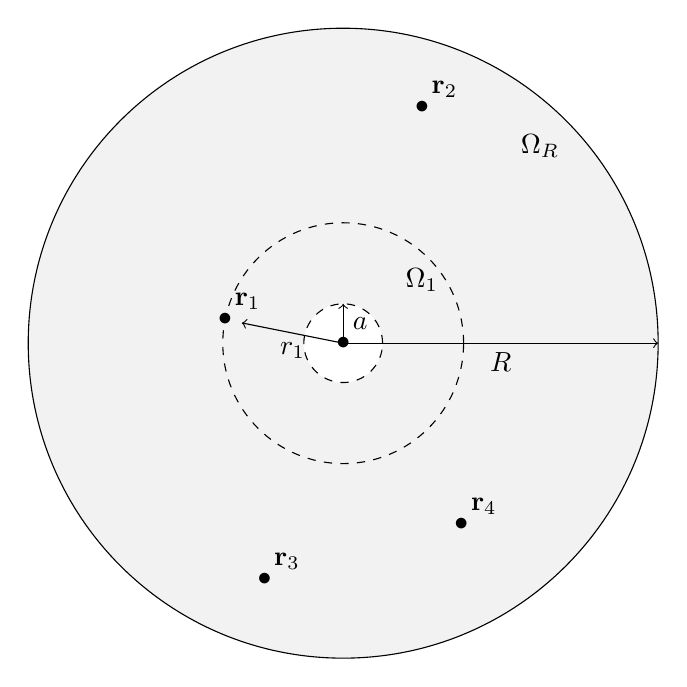
\begin{tikzpicture}
        \draw[fill=gray!10] (0,0) circle (4);
        \draw[dashed,fill=white] (0,0) circle (0.5);
        \draw[->](0,0)--(4,0)node[midway,below]{$R$};
        \draw[->](0,0)--(0,0.5)node[midway,right]{$a$};
        \node (O) at (0,0){$\bullet$}; 
        \node (r1) at (-1.5,0.3){$\bullet$}; 
        \node (r2) at (1,3){$\bullet$}; 
        \node (r3) at (-1,-3){$\bullet$}; 
        \node (r4) at (1.5,-2.3){$\bullet$}; 
        \draw (r1) node [above right] {$\textbf{r}_1$};
        \draw (r2) node [above right] {$\textbf{r}_2$};
        \draw (r3) node [above right] {$\textbf{r}_3$};
        \draw (r4) node [above right] {$\textbf{r}_4$};
        \draw[->] (0,0) -- (r1) node [midway, below] {$r_1$};
        \node  at (2.5,2.5){$\Omega_R$}; 
        \draw[dashed] (0,0) circle (1.529);
        \node  at (1,0.8){$\Omega_1$}; 
    \end{tikzpicture}
\end{figure}
We assume that, 
\begin{itemize}
    \item The number of droplets /particles in the domain is constant and is noted $N$. 
    Droplets might rise and go out the domain however we assume that the same number go inside at the same time as the domain is supposed either physical or periodic, or large enough. 
    \item The size of the domain $\Omega_R$ is $4/3 \pi R^3$
    \item All the length can be made dimensionless with the radius of a droplet noted $a$.
\end{itemize}


\subsubsection{Decomposition of the 2points nearest particle statistics probability}

We search to compute the probability distrbution $P_\text{2-nst-f}[\textbf{r}_1,\textbf{r}_2,\textbf{x}]$ defined as, 
\begin{align}
    \phi_f
    &= 
    \avg{\chi_f}\\
    \phi_f P^f_1
    &= 
    \avg{\chi_f \sum_{i=1}^{N}\delta(\textbf{x}_i - \textbf{x} - \textbf{r})}\\
    \phi_f P_\text{nst}^f =
    \phi_f P_1^f h_\text{nst}^\text{1-f}
    &= 
    \avg{\chi_f  
    \sum_i^N \delta(\textbf{x}_i - \textbf{x}- \textbf{r})
    h_i
    }\\
    \phi_f P_\text{2-nst}^f
    &= 
    \avg{\chi_f  
    \sum_i^N \delta(\textbf{x}_i - \textbf{x}- \textbf{r})
    h_i
    \sum_{j\neq i}^N \delta(\textbf{x}_j - \textbf{x}- \textbf{r})
    h_j
    }
\end{align}

This distribution can be decomposed as, 
\begin{equation}
    P_\text{nst-f-2}
    =
    \phi_f
    P_\text{nst}^f
    P_\text{2-nst}^\text{nst-f}
\end{equation}
Each of these distributions can then be decomposed as, 
\begin{align}
    P_\text{nst}^f
    &=
    P_\text{1}^f
    h^\text{1-f}_\text{nst}\\
    P_\text{2-nst}^\text{nst-f}
    &=
    P_\text{2}^\text{nst-f}
    h^\text{2-f}_\text{nst}
\end{align}
where, 
\begin{itemize}
    \item $P_\text{1}^f$ is the probability of finding a particle at $\textbf{r}_1$ knowing the continuous phase is at $\textbf{x}$
    \item $h^\text{1-f}_\text{nst}$ is the probability that the particle at $\textbf{r}_1$ is the nearest one to the point \textbf{x} knowing that there is indeed a particle at $\textbf{r}_1$ and the fluid at \textbf{x}. 
    \item $P_\text{2}^\text{nst-f}$ is the probability of finding a particle at $\textbf{r}_2$ knowing the continuous phase is at $\textbf{x}$ and the nearest particle to \textbf{x} is at $\textbf{r}_1$. 
    \item $h^\text{2-f}_\text{nst}$ is the probability that the particle at $\textbf{r}_2$ is the second-nearest one to the point \textbf{x} knowing that there is indeed a particle at $\textbf{r}_1$ and the fluid at \textbf{x}. 
\end{itemize}

\subsubsection{Unconditional number density}
The probability of finding a particle center of mass in a small element $d\textbf{x}$ around a point \textbf{x} is, 
\begin{equation}
    n_p(\textbf{x}+ \textbf{r})
    = \avg{\sum_{i=1}^N \delta(\textbf{x}-\textbf{x}_i[\FF,t])}
    =
    \frac{N}{\frac{4}{3}\pi R^3}
    \;\;\;\; \forall |\textbf{r}| = r < R  
\end{equation}
Additionally we can define the volume fraction, 
\begin{equation}
    \phi = 4/3 \pi a^3 n_p
\end{equation}
\subsubsection{One point conditioned particle statistics}

At the first level or accuracy we stipulate that the number density at a given point \textbf{x}+\textbf{r} within $\Omega_R$ knowing that the continuous phase is at \textbf{x} can be defined as, 
\begin{equation}
    P_\text{1}^f(\textbf{x}+ \textbf{r})
    = \avg{\sum_{i=1}^N \delta(\textbf{x}-\textbf{x}_i[\FF,t])}
    =
    \frac{N}{\frac{4}{3}\pi R^3 (1 - (a/R)^3)}
    =
    \frac{n_p}{ (1 - (a/R)^3)}
    \;\;\;\; \forall a< r < R   
\end{equation}
The second equality is determined using ``ergodic'' assumption. 

The probability $h^\text{1-f}_\text{nst}$ is the probability of finding no particle in the domain, $\Omega_1$. 
The methodology is  as follow,
(1) The probability of finding a particle in the infinitesimal portion of the volume $V_1$ is $P^\text{1-f}_1 dV_1$ where $dV_1 = V_1 / n$ for $n\in \mathbb{N}$. 
(2) $P^\text{1-f}_1$ is the number density of particles conditioned on that the nearest particles to the point \textbf{x} is at $\textbf{r}_1$, thus, 
\begin{equation}
    P^\text{nst-f}_1
    =
    \frac{N - 1}{\frac{4}{3}\pi R^3 (1 - (r_1/R)^3)}
    % \approx
    % \frac{N_v }{\frac{4}{3}\pi R^3 (1 - (r_1/R)^3)}
    = 
     \frac{n_p - \frac{3}{4 \pi R^3}}{1 - (r_1/R)^3}
\end{equation} 
(3) The probability of finding no particles in any of these $n$ subdomain is $(1 - V_1 P^\text{nst-f}_1 /n)^n$, hence, 
\begin{equation}
    h^\text{1-f}_\text{nst}
    =
    \lim_{n\to\infty}
    (1 - \frac{V_1 P^\text{nst-f}_1}{n})^n
    =
    e^{-P^\text{nst-f}_1 V_1 }
    =
    e^{- \frac{\phi - \frac{a^3}{ R^3}}{1 - (r_1/R)^3}  (r_1^3 - 1) }
\end{equation}


Hence, the probability $P_\text{nst}^f$ is defined as, 
\begin{equation}
    P_\text{nst}^f
    =
    \frac{3 a^3}{4 \pi}\frac{\phi}{ (1 - (a/R)^3)}
    e^{- (\phi - \frac{a^3}{ R^3})\frac{(r_1^3 - 1)}{1 - (r_1/R)^3}   }
\end{equation}
Making all the length dimensionless with the particles radius gives 
\begin{equation}
    P_\text{nst}^f
    =
    \frac{3 }{4 \pi}\frac{\phi}{ 1 - 1/R^3}
    e^{- \phi \frac{r_1^3 -1 }{1 - (r_1/R)^3}}
\end{equation}